\section{Appendix - Design drawings}
\section{Appendix - Model}
\label{AppendixModel}

\subsection{Cross-sections}

\subsection{Hangers}
\label{Appendix_A_Hangers}

\subsection{Live loading} \label{Appendix_Liveloading}
In this chapter, the arrangement of the live loads on the deck is investigated. The three design states ultimate limit state, hanger replacement and hanger loss are treated individually as different circumstances apply to them. In a first step, the location of each lane is defined. The width according to [AASHTO] is always equal to $\SI{12}{ft} = \SI{3.7}{m}$ of which \SI{3}{m} are loaded and the centroid of the applied forces $x_c$ can be derived. The force applied to the tie girder $F_r$ can then be calculated according to Eq. \ref{eq:reaction} using the width of the deck $w_{deck}=\SI{107}{ft}=\SI{32.6}{m}$.
\begin{equation}
    F_r = \frac{x_c}{w_{deck}}
    \label{eq:reaction}
\end{equation}
In a second step, the amount of loaded lanes is determined. As the multiple presence factors (MPF) decrease with the amount of loaded lanes, each possibility is calculated to find the worst arrangement. The calculations are conducted for a unit lane load. The obtained factor relates the load on one lane to the load that is applied on the investigated tie girder. The factor can then be used for the calculation of the force on the tie of the distributed lane load ($q_{LL}=\SI{9.3}{kN/m}$) as well as of the design truck load ($Q_{LL}=\SI{325}{kN}$). For the design truck load an additional dynamic multiplier of 1.33 is taken into account. 

\subsubsection{Ultimate limit state} \label{Appendx_A_Live_loading_1}
In the ultimate limit state, the entire width of the deck is available to traffic. The lanes are arranged as densely to one side as possible and the first lane starts at $\SI{4.6}{ft}=\SI{1.4}{m}$ from the investigated arch plane. The calculations presented in Table \ref{tab:app_ll_uls} show that the worst arrangement results with six loaded lanes. 

\begin{table}[H]
\centering
\begin{tabular}{cccccccccccc}
\cline{2-11}
             & Lane     &  & 1    & 2    & 3    & 4    & 5    & 6    & 7    & 8    &      \\
             & Centroid &  & 2.9  & 6.6  & 10.2 & 13.9 & 17.5 & 21.2 & 24.8 & 28.5 &      \\
             & Reaction &  & 0.91 & 0.80 & 0.69 & 0.57 & 0.46 & 0.35 & 0.24 & 0.13 &      \\ \hline
Loaded Lanes & MPF      &  &      &      &      &      &      &      &      &      & Sum  \\ \hline
1            & 1.2      &  & 1.09 &      &      &      &      &      &      &      & 1.09 \\
2            & 1.0      &  & 0.91 & 0.80 &      &      &      &      &      &      & 1.71 \\
3            & 0.85     &  & 0.77 & 0.68 & 0.58 &      &      &      &      &      & 2.04 \\
4            & 0.75     &  & 0.68 & 0.60 & 0.52 & 0.43 &      &      &      &      & 2.23 \\
5            & 0.70     &  & 0.64 & 0.56 & 0.48 & 0.40 & 0.32 &      &      &      & 2.40 \\
6            & 0.65     &  & 0.59 & 0.52 & 0.45 & 0.37 & 0.30 & 0.23 &      &      & 2.46 \\
7            & 0.60     &  & 0.55 & 0.48 & 0.41 & 0.34 & 0.28 & 0.21 & 0.14 &      & 2.41 \\
8            & 0.55     &  & 0.50 & 0.44 & 0.38 & 0.32 & 0.25 & 0.19 & 0.13 & 0.07 & 2.28 \\ \hline
\end{tabular}
\caption{Force on tie girder for ultimate limit state under unit lane load}
\label{tab:app_ll_uls}
\end{table}

It can be seen that six loaded lanes yield a factor of 2.46. Hence the load applied on the investigated arch plane can be calculated according to Eqs. \eqref{eq:q_ll_uls} and \eqref{eq:Q_ll_uls}. The decisive arrangement is illustrated in Fig. \ref{fig:app_hangers_uls}.
\begin{equation}
    q_{ll, uls} = 2.46 \cdot \SI{9.3}{kN/m} = \SI{22.9}{kN/m}
    \label{eq:q_ll_uls}
\end{equation}
\begin{equation}
    Q_{ll, uls} = 2.46 \cdot 1.33 \cdot \SI{325}{kN} = \SI{1063}{kN}
    \label{eq:Q_ll_uls}
\end{equation}

\begin{figure}[H]
    \centering
    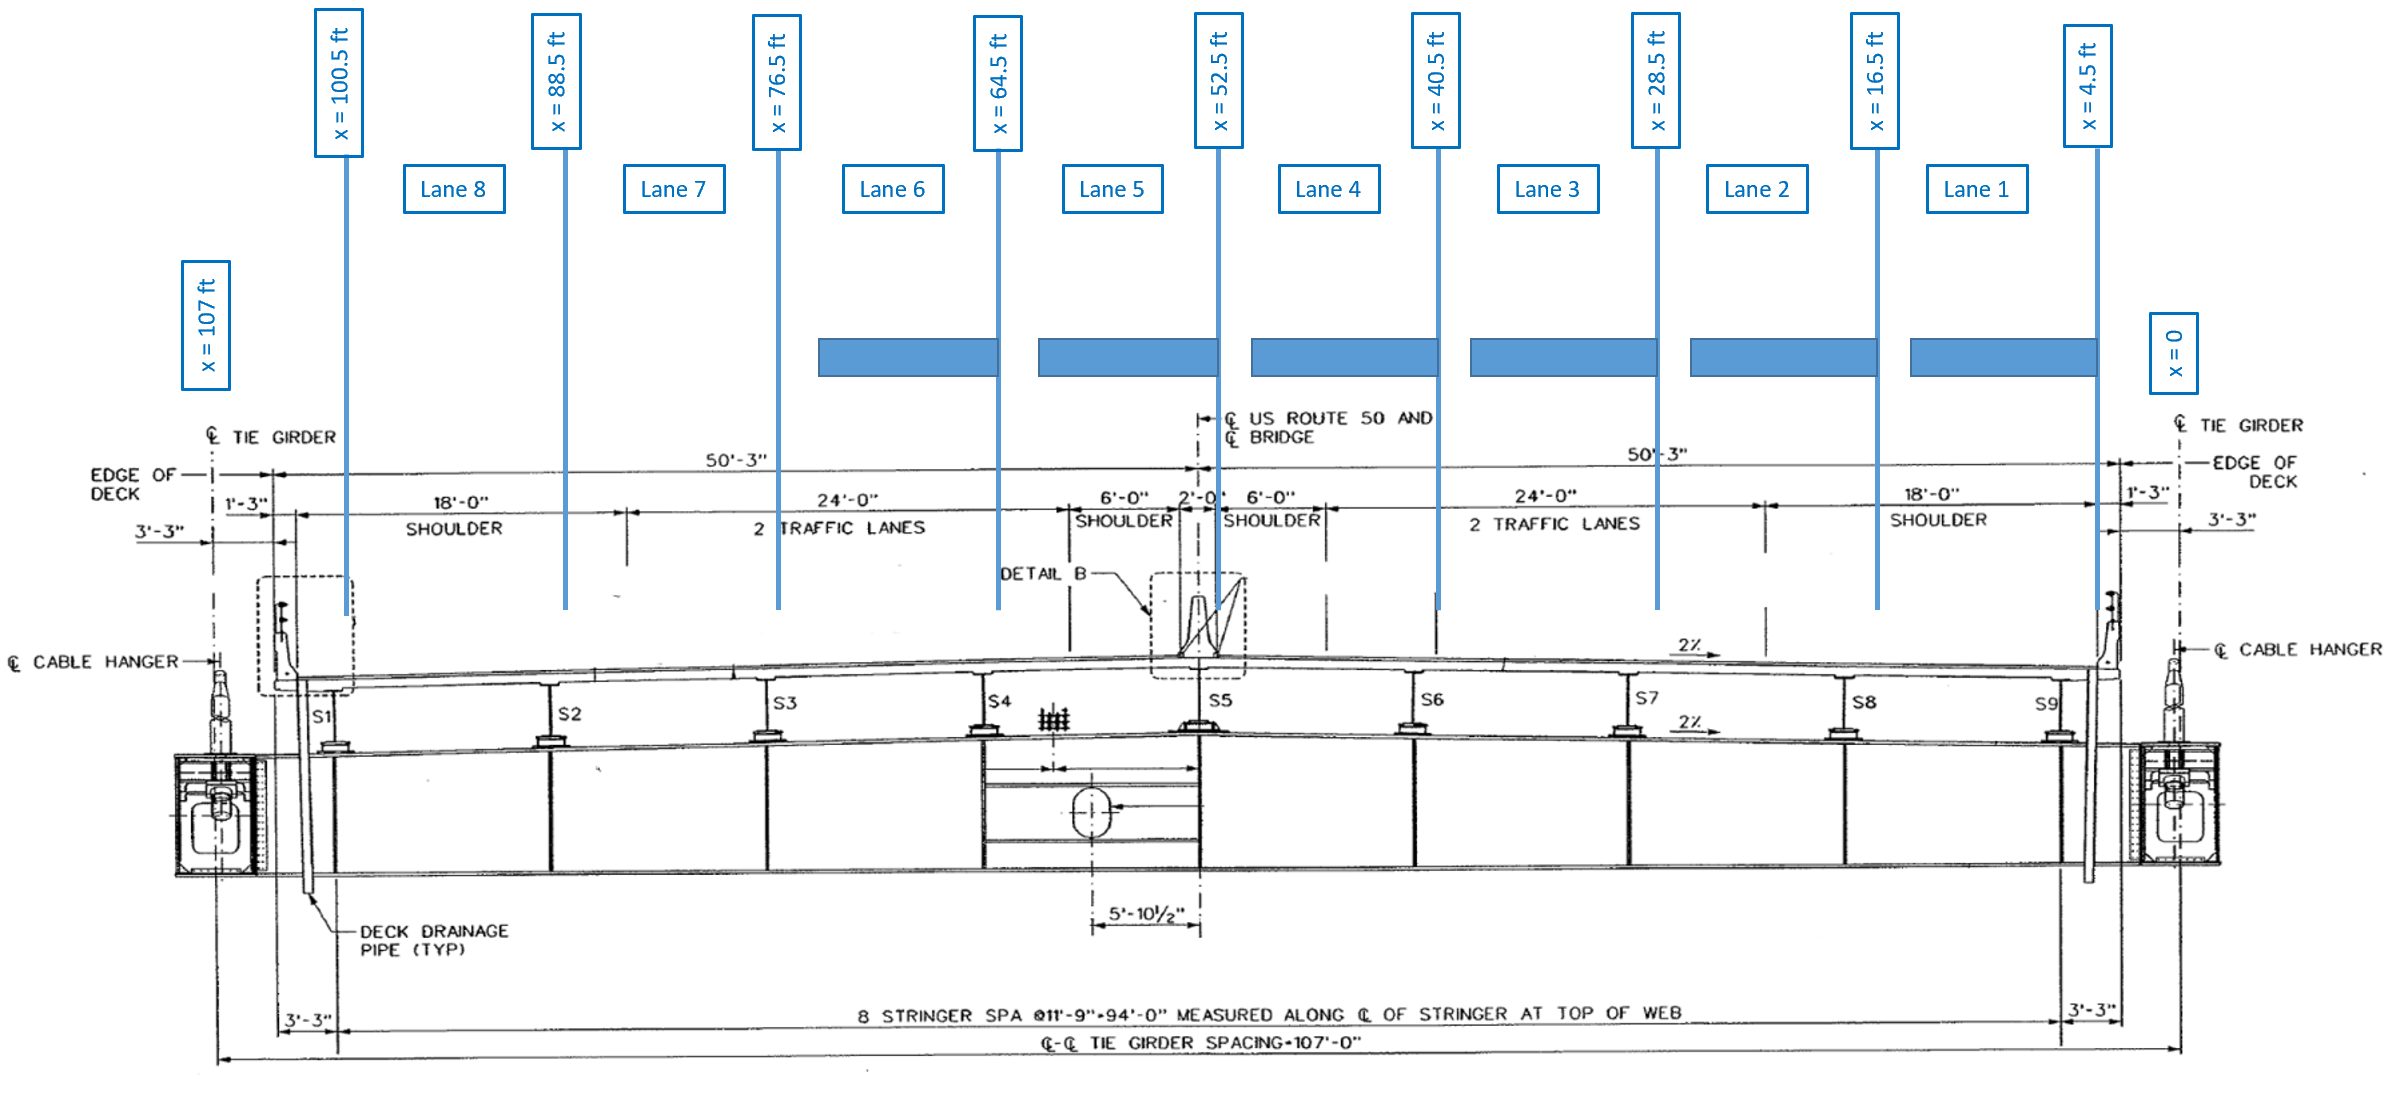
\includegraphics[width=0.9\textwidth]{overleaf/Appendix/Pictures/Cross_Section_LL_ULS.PNG}
    \caption{Illustration of the live load arrangement in the ultimate limit state}
    \label{fig:app_hangers_uls}
\end{figure}




\subsubsection{Hanger replacement} \label{Appendx_A_Live_loading_2}
In the event of hanger replacement, one lane is shifted away from the hanger being exchanged. Besides that the lanes are located at the same positions as in the ultimate limit state. A load for the replacement truck is disregarded for in this investigation. The calculation of the different arrangements is presented in Table \ref{tab:app_ll_hanger_replacement}.
\begin{table}[H]
\centering
\caption{Force on tie girder for hanger replacement under unit lane load}
\label{tab:app_ll_hanger_replacement}
\resizebox{.8\textwidth}{!}{%
\begin{tabular}{cccccccccccc}
\cline{2-11}
             & Lane     &  & 1    & 2    & 3    & 4    & 5    & 6    & 7    & 8    &      \\
             & Centroid &  & 2.9  & 6.6  & 10.2 & 13.9 & 17.5 & 21.2 & 24.8 & 28.5 &      \\
             & Reaction &  & 0.91 & 0.80 & 0.69 & 0.57 & 0.46 & 0.35 & 0.24 & 0.13 &      \\ \hline
Loaded Lanes & MPF      &  &      &      &      &      &      &      &      &      & Sum  \\ \hline
1            & 1.2      &  & -    & 0.96 &      &      &      &      &      &      & 0.96 \\
2            & 1.0      &  & -    & 0.80 & 0.69 &      &      &      &      &      & 1.49 \\
3            & 0.85     &  & -    & 0.68 & 0.58 & 0.49 &      &      &      &      & 1.75 \\
4            & 0.75     &  & -    & 0.60 & 0.52 & 0.43 & 0.35 &      &      &      & 1.89 \\
5            & 0.70     &  & -    & 0.56 & 0.48 & 0.40 & 0.32 & 0.25 &      &      & 2.01 \\
6            & 0.65     &  & -    & 0.52 & 0.45 & 0.37 & 0.30 & 0.23 & 0.15 &      & 2.02 \\
7            & 0.60     &  & -    & 0.48 & 0.41 & 0.34 & 0.28 & 0.21 & 0.14 & 0.08 & 1.94 \\ \hline
\end{tabular}
}
\end{table}

The resulting loads on the investigated arch plane are presented in Eqs. \eqref{eq:q_ll_repl} and \eqref{eq:Q_ll_repl}
\begin{equation}
    q_{ll, repl} = 2.02 \cdot \SI{9.3}{kN/m} = \SI{18.8}{kN/m}
    \label{eq:q_ll_repl}
\end{equation}
\begin{equation}
    Q_{ll, repl} = 2.02 \cdot 1.33 \cdot \SI{325}{kN} = \SI{874}{kN}
    \label{eq:Q_ll_repl}
\end{equation}

\newpage
\subsubsection{Hanger loss} \label{Appendx_A_Live_loading_3}
In the extreme event of hanger loss, not the entire width of the deck is available to the live loads. For this case, only the four actually marked lanes are available. Their locations were taken from the design drawings. The investigation in Table \ref{tab:app_ll_cable_loss} shows that all of these lanes are loaded in the worst arrangement.
\begin{table}[H]
\centering
\caption{Force on tie girder for cable loss under unit lane load}
\label{tab:app_ll_cable_loss}
\begin{tabular}{cccccccc}
\cline{2-7}
             & Lane     &  & 1    & 2    & 3    & 4    &      \\
             & Centroid &  & 8.4  & 12.0 & 20.0 & 23.6 &      \\
             & Reaction &  & 0.74 & 0.63 & 0.39 & 0.28 &      \\ \hline
Loaded Lanes & MPF      &  &      &      &      &      & Sum  \\ \hline
1            & 1.2      &  & 0.89 &      &      &      & 0.89 \\
2            & 1.0      &  & 0.74 & 0.63 &      &      & 1.37 \\
3            & 0.85     &  & 0.63 & 0.54 & 0.33 &      & 1.50 \\
4            & 0.75     &  & 0.56 & 0.47 & 0.29 & 0.21 & 1.53 \\ \hline
\end{tabular}
\end{table}

The loads resulting on the tie girder are calculated in Eqs. \eqref{eq:q_ll_loss} and \eqref{eq:Q_ll_loss}
\begin{equation}
    q_{ll, loss} = 1.53 \cdot \SI{9.3}{kN/m} = \SI{14.2}{kN/m}
    \label{eq:q_ll_loss}
\end{equation}
\begin{equation}
    Q_{ll, loss} = 1.42 \cdot 1.33 \cdot \SI{325}{kN} = \SI{660}{kN}
    \label{eq:Q_ll_loss}
\end{equation}

An illustration of the load arrangement for the event of cable loss is presented in Fig. \ref{fig:app_hangers_cable_loss}.

\begin{figure}[H]
    \centering
    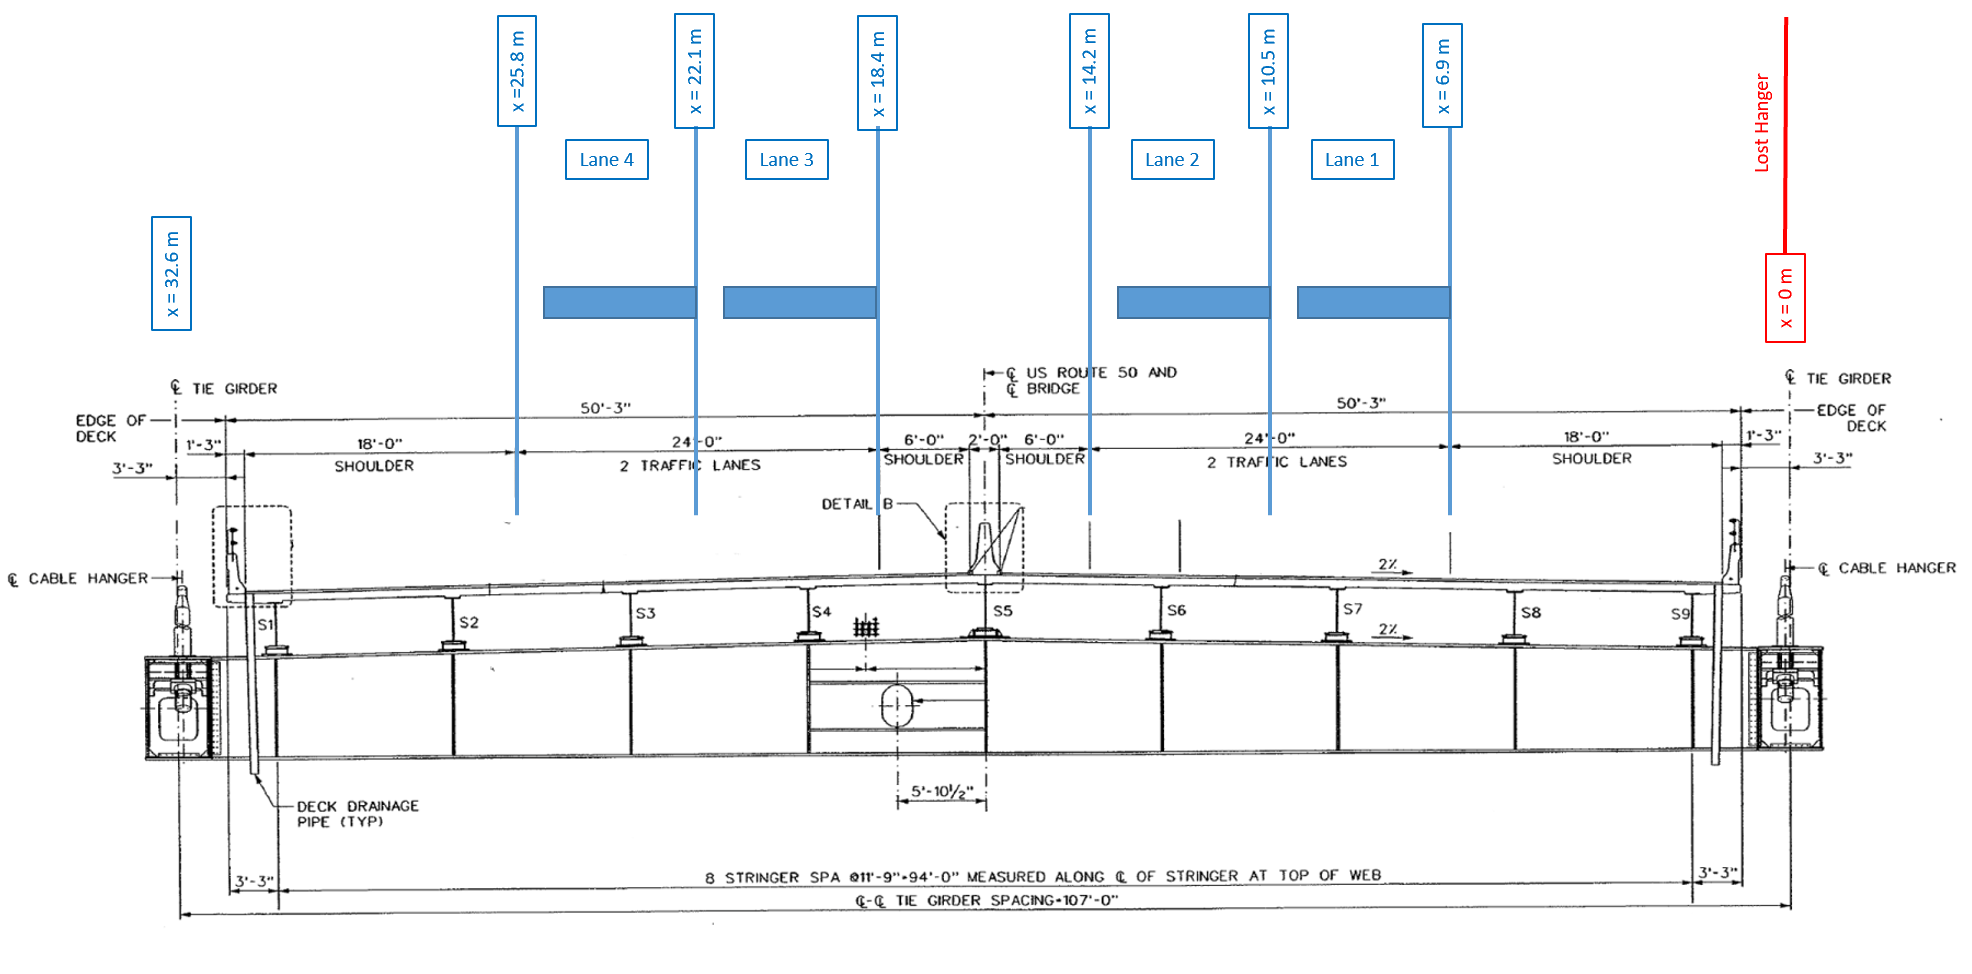
\includegraphics[width=0.9\textwidth]{overleaf/Appendix/Pictures/Cross_Section_LL_Cable Loss.PNG}
    \caption{Illustration of the live load arrangement for hanger loss}
    \label{fig:app_hangers_cable_loss}
\end{figure}

\section{Optimisation methods}

\section{Implementation}

